\experiment{Linear Search}{29/11/2023}

\section{Aim}
To make a program that inputs and stores empolyee details such as id, name and salary. Implement linear search to search employee details with the given empolyee id.

\section{Algorithm}
 {\fontfamily{lmtt}\selectfont

  \subsection{Employee Structure}
  \begin{enumerate}[label=\arabic*:,left=0pt]
    \item \textbf{Start}
    \item Define a structure for an employee:
          \begin{enumerate}[label=2.\arabic*.]
            \item Include \texttt{id} (integer), \texttt{name} (character array), and \texttt{salary} (integer).
          \end{enumerate}
    \item \textbf{Stop}
  \end{enumerate}

  \subsection{Main Function}
  In the \texttt{main} function:
  \begin{enumerate}[label=\arabic*:, start=1]
    \item \textbf{Start}
    \item Print "Enter the number of employees: ".
    \item Take user input for \texttt{n}.
    \item Allocate memory for an array of employees (\texttt{arr}) using \texttt{malloc(n * sizeof(employee))}.
    \item Loop from \texttt{i} equal to 0 to \texttt{n - 1}:
          \begin{enumerate}[label=4.\arabic*:, start=1]
            \item Print "Enter the id, name, and salary of employee \texttt{i + 1}: ".
            \item Take user input for \texttt{arr[i].id}, \texttt{arr[i].name}, and \texttt{arr[i].salary}.
          \end{enumerate}
    \item Print "Enter the id of the employee to search: ".
    \item Take user input for \texttt{id}.
    \item Loop from \texttt{i} equal to 0 to \texttt{n - 1}:
          \begin{enumerate}[label=8.\arabic*:, start=1]
            \item Check if \texttt{arr[i].id} is equal to \texttt{id}:
                  \begin{enumerate}[label=8.1.\arabic*:, start=1]
                    \item Print "Employee found".
                    \item Print "Id:", \texttt{arr[i].id}.
                    \item Print "Name:", \texttt{arr[i].name}.
                    \item Print "Salary:", \texttt{arr[i].salary}.
                    \item Return 0.
                  \end{enumerate}
          \end{enumerate}
    \item Print "Employee not found".
    \item \textbf{Stop}
  \end{enumerate}
  \textbf{End Algorithm}
 }

\section{C Program}
\begin{lstlisting}[label={list:c_program:employee_search}]
#include <stdio.h>
#include <stdlib.h>

typedef struct employee
{
  int id;
  char name[100];
  int salary;
} employee;

int main()
{
  printf("Enter the number of employees: ");
  int n;
  scanf("%d", &n);
  employee *arr = (employee *)malloc(n * sizeof(employee));
  for (int i = 0; i < n; i++)
  {
    printf("\nEnter the id, name and salary of employee %d: ", i + 1);
    scanf("%d %s %d", &arr[i].id, arr[i].name, &arr[i].salary);
  }
  printf("\nEnter the id of the employee to search: ");
  int id;
  scanf("%d", &id);
  for (int i = 0; i < n; i++)
  {
    if (arr[i].id == id)
    {
      printf("\nEmployee found\n");
      printf("Id: %d\nName: %s\nSalary: %d\n", arr[i].id, arr[i].name, arr[i].salary);
      return 0;
    }
  }
  printf("\nEmployee not found\n");
}
\end{lstlisting}

\section{Output}
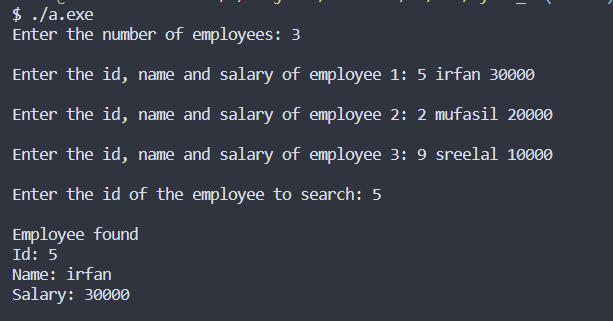
\includegraphics[]{Cycle_1/Outputs/LinearSearch.png}

\section{Result}
Program is executed and output is verified